\section{Metodología}
\subsection{Arquitecturas entrenadas}
La MLP aplica Flatten, Dense256/ReLU, dropout 0.5 y Dense104; tiene 9,660,776
parámetros. La primera capa aporta 9,634,048 (99.72\%), porque cada uno de los
37,632 valores de entrada se conecta con las 256 unidades, además de sus sesgos.
No contiene convoluciones ni pooling.

La CNN original contiene cuatro Conv $3\times3$, padding \textit{same}, con
32, 64, 128 y 256 filtros, ReLU y max pooling $2\times2$ por bloque. Las salidas
son $56\times56\times32$, $28\times28\times64$, $14\times14\times128$ y
$7\times7\times256$. GAP, Dense256/ReLU, dropout 0.5 y Dense104 completan
480,936 parámetros. La CNN ampliada añade Conv128 después de pool3 y Conv256
después de pool4, ambas $3\times3$/ReLU, sin pool adicional: seis convoluciones
y 1,218,600 parámetros. La variante AdamW/LR conserva la arquitectura original.
\begin{figure*}[htbp]
\centering
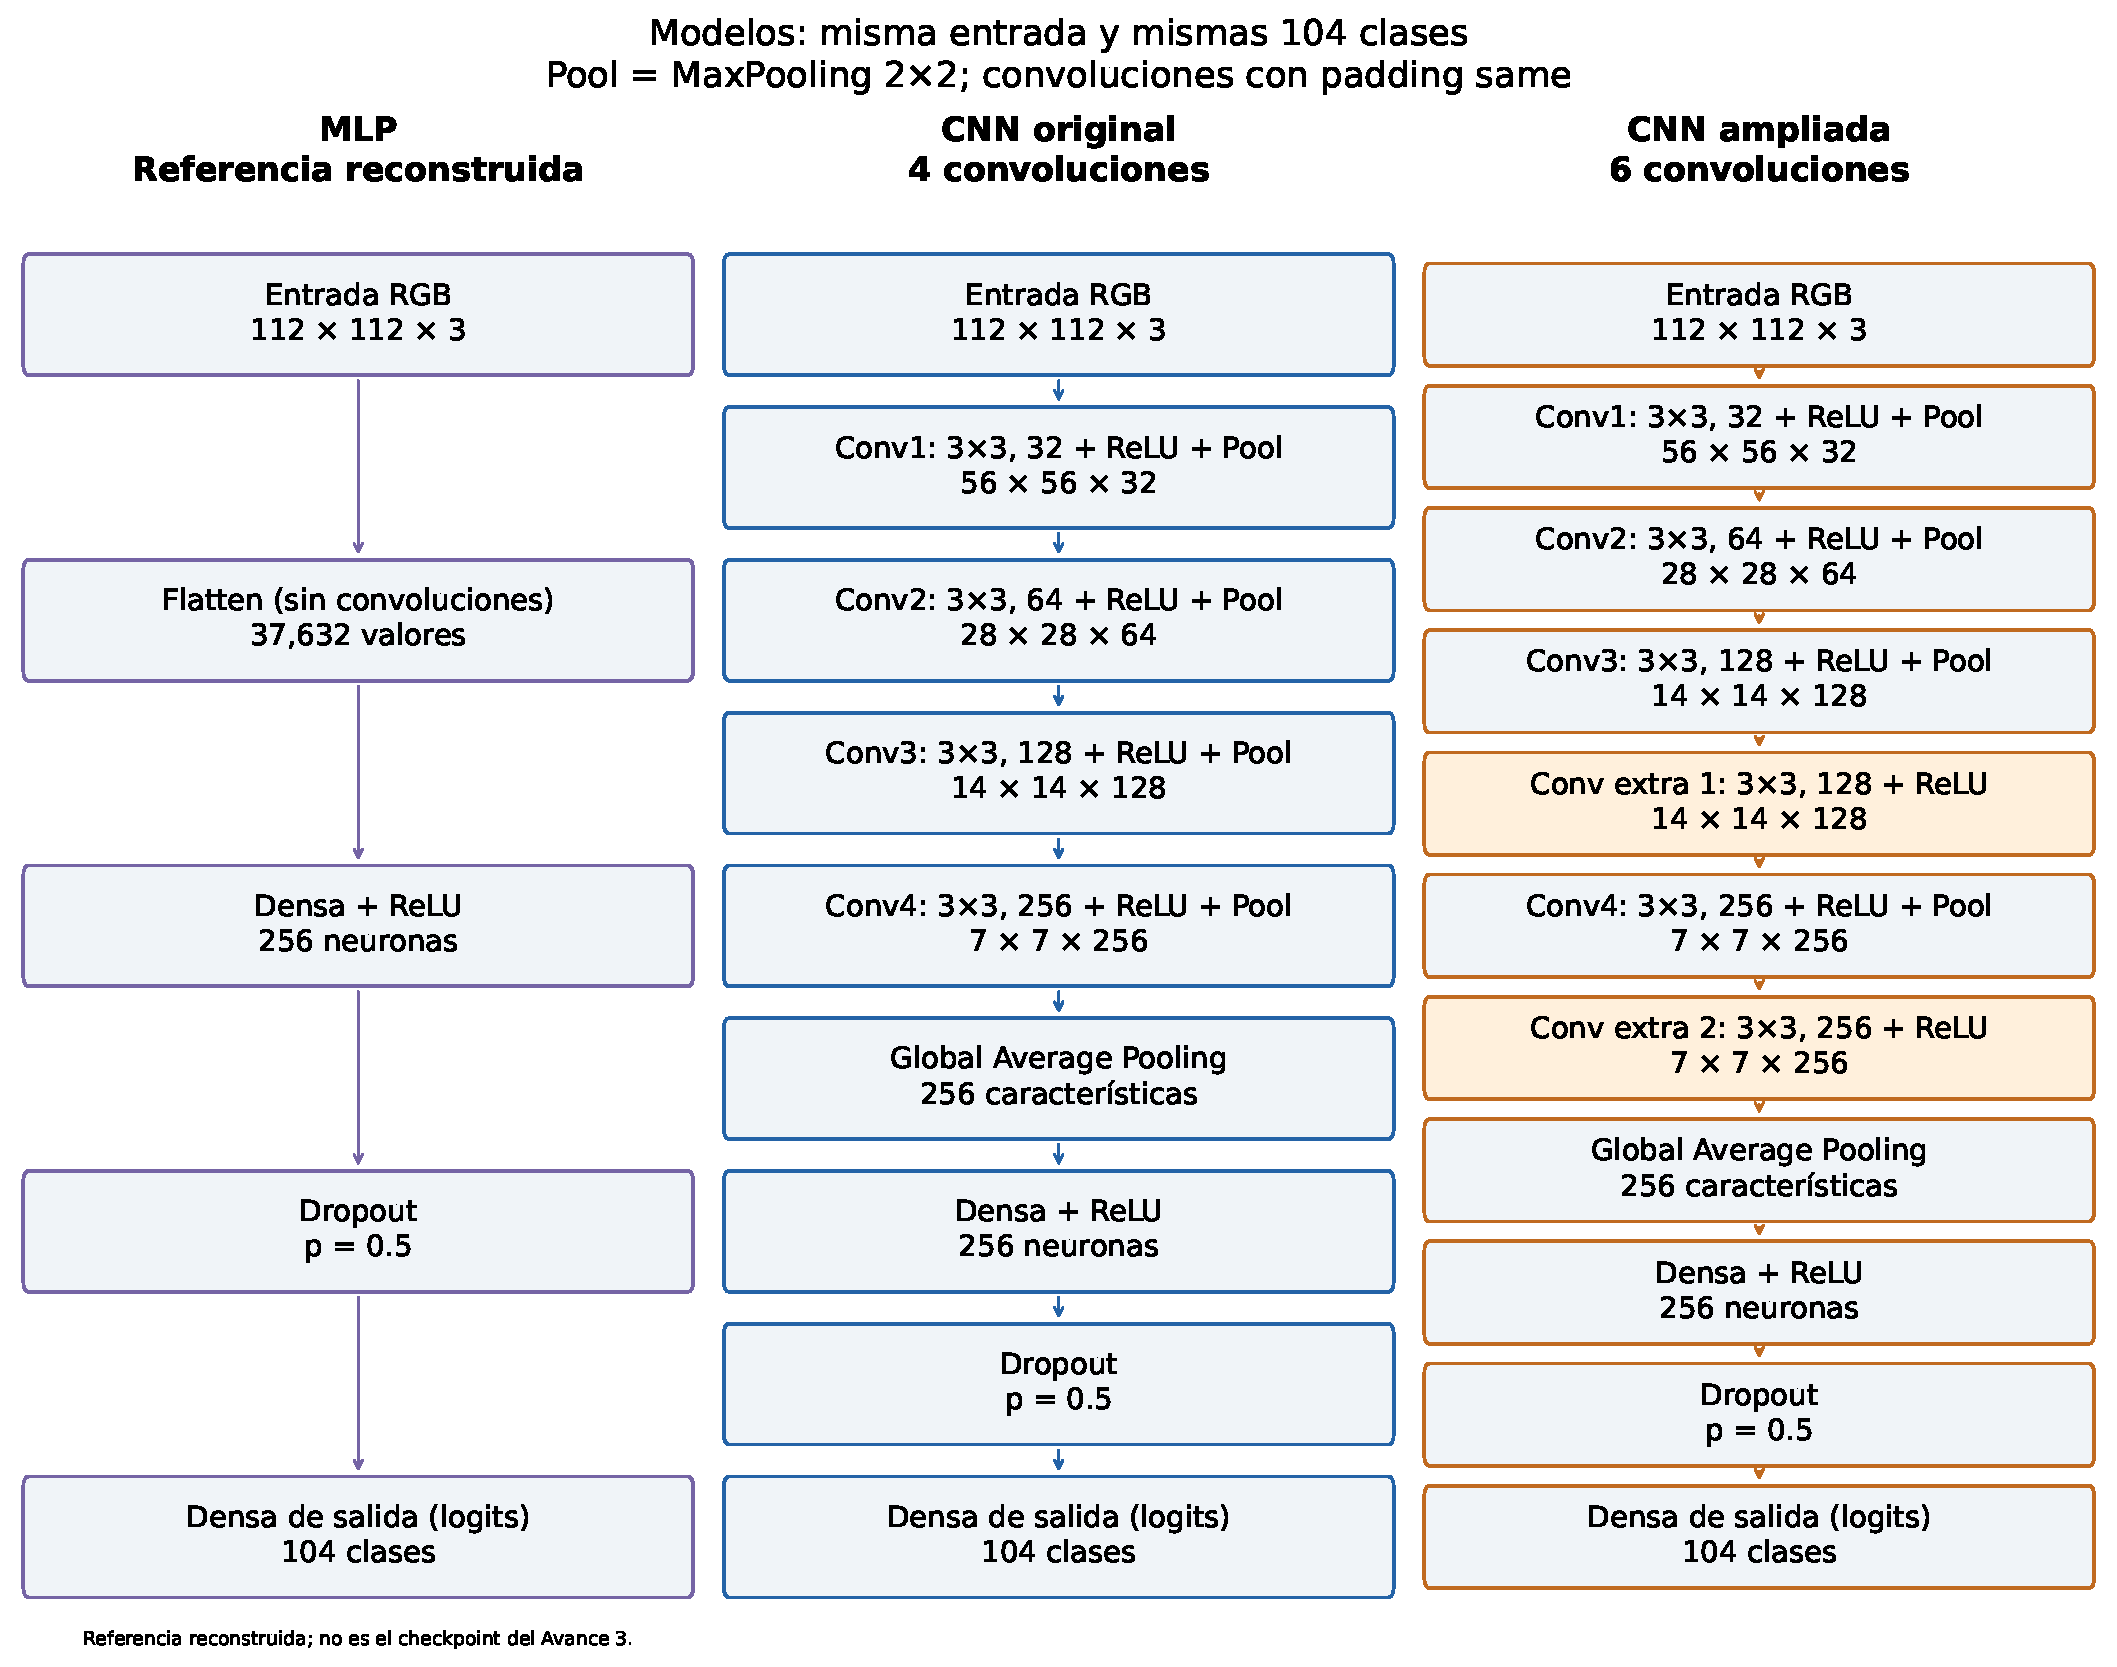
\includegraphics[width=0.93\textwidth,height=0.65\textheight,keepaspectratio]{avance4_2026-10-21/figures/arquitecturas.pdf}
\caption{Arquitecturas históricas A4 con entrada efectiva de 112 por 112. Las capas
adicionales de la CNN ampliada se muestran en naranja.}\label{fig:arquitecturas-av4}
\end{figure*}

\subsection{Preprocesamiento}
El lector decodifica JPEG RGB, convierte a float32, divide por 255 y redimensiona
con interpolación bilineal y antialias a $112\times112$. Train se mezcla y usa
volteo horizontal, rotación de factor 0.05, zoom 0.1 y contraste 0.1; los valores
se recortan a $[0,1]$. La caché precede a los aumentos, que cambian entre épocas.
Validación no usa transformaciones aleatorias. La MLP aplana en orden NHWC,
coherente entre su implementación PyTorch y la exportación Keras.

\subsection{Implementación y procedencia}
Las cuatro corridas A4 se entrenaron históricamente con PyTorch/DirectML en
Radeon RX 6700S y lector TensorFlow; sus checkpoints PT se exportaron a Keras.
Los registros conservan una prueba histórica de paridad sobre un lote. Este
análisis recalcula métricas desde las predicciones guardadas y coteja las pérdidas
con los archivos; no vuelve a ejecutar inferencia sobre imágenes.

El par complementario F procede del reporte final y utiliza TensorFlow/Metal,
según su documentación. No se trata de una repetición DirectML. La destilación
Distribution Matching pertenece a otro experimento del proyecto: no se usaron
sus imágenes sintéticas para entrenar las seis corridas aquí comparadas.
